\documentclass[a4paper,12pt]{report}
\usepackage[utf8]{inputenc}
\usepackage{graphicx}
\usepackage[document]{ragged2e}

\begin{document}
\title{Rapport Intelligence Artificielle}

\author{\texttt{Charlotte Rodriguez}\\
		\texttt{Borjan Geshkovski}\\
		\texttt{Naomie Terral}
		}
\maketitle

\section{Introduction à l'intelligence artificielle}

\subsection{L'intelligence artificielle et ses enjeux}
\ \ \ \ \ L'intelligence artificielle est un domaine de l'informatique consacré au développement de programmes, permettant aux ordinateurs d'avoir un comportement que l'on peut caractériser d'intelligent. La majeur partie de la recherche en intelligence artificielle est focalisée sur des applications extrêmement précises, telles que la prise de décision, la perception, l'adaptation à un nouvel environnement, la mémoire... \\
Un des buts principaux de l'intelligence artificielle est de construire des entités intelligentes autonomes, capable d'exécuter des tâches complexes à la portée de l'être humain ou non. \\ 
Dans la communauté informatique, on observe des divergences d'opinions, quant aux objectifs de l'intelligence artificielle. 
\begin{itemize}
\item Doit-elle avoir seulement l'apparence de l'intelligence? (Intelligence artificielle forte)
\item Son fonctionnement interne doit-il être semblable à celui de l'être humain, et être au moins aussi rationnel ? (Intelligence artificielle faible)
\end{itemize}
Dans le cadre de ce projet, nous nous situons plutôt dans le domaine de l'intelligence artificielle faible, en cherchant à reproduire le mécanisme de la prise de décision de l'être humain. \\
\ \ \ \ \ L'intelligence artificielle s'est illustrée, au cours du temps dans différentes applications. \\
On a pu observer des utilisations de l'intelligence artificielle dans les jeux de stratégie (nécessitant une prise de décision).
Un des événements les plus marquants des ces 30 dernières années, est la victoire de Deep Blue (superordinateur conçu par IBM), sur le champion du monde d'échec des années 90, Garry Kasparov. On se rappelle aussi de la victoire de Watson (aussi conçu par IBM), au jeu télévisé Jeopardy!, en 2011. Encore plus récemment, en 2015, le logiciel AlphaGo, créé par Google a battu le triple champion européen de jeu de Go.
\\
Une autre application intéressante est le développement de chatbots, comme est l'exemple d'ELIZA, codé par Joseph Weizenbaum dans les années 60. Elle simule un dialogue actif entre un psychothérapeute (ordinateur) et son patient(utilisateur). C'est un intelligence artificielle, au sens de l'intelligence artificielle faible, puisqu'elle ne comprend pas ce que l'interlocuteur lui dit, et ses réponses sont construites à partir de modèles pré-établis et de mots clés identifiés dans l'entrée de l'utilisateur.
\\
Il y a quelques mois, Microsoft a subit un lourd échec avec le chatbot TAY, un compte Twitter simulant le langage d'une jeune adulte de 19 ans, dans le but d'apprendre à interagir avec les utilisateurs de ce réseaux social. \\
Quels sont les enjeux de l'intelligence artificielle ? 



\subsection{Le problème}
\ \ \ \ \ Dans ce rapport nous tendons d'aborder la question de la prise de décision, élément central à l'intelligence artificielle. Nous abordons cette problématique, selon trois points de vue différents : celui d'un agent autonome, celui d'un consommateur, et celui d'une entreprise. \\
Avant de poursuivre plus, définissons les notions d'agent et de prise de décision. \\
Un agent est " une entité autonome, ca pable de percevoir son environnement grâce à des capteurs, et aussi d'agir sur celui-ci via des effecteurs afin de réaliser des buts. Un agent peut également apprendre et utiliser des connaissances pour pouvoir réaliser ses objectifs"\footnote{Stuart Russel et Peter Norvige, Intelligence Artificielle, 2012}.\\
Dans ce projet, l'agent est un aspirateur plus ou moins intelligent (il ne disposera pas obligatoirement de capteurs). Nous étudions trois classes d'aspirateurs : 
\begin{itemize}
\item Un aspirateur aléatoire
\item Un aspirateur disposant d'une base de règle, associée à la possibilité d'apprentissage
\item Un aspirateur dit "génétique", dont le comportement est déterminé par un algorithme d'optimisation (algorithme génétique)
\end{itemize}
On entend par prise de décisions le processus qui consiste à faire un choix parmi plusieurs alternatives.
Dans le dictionnaire, une prise de décision est définie comme un processus cognitif complexe consistant en un choix d'action parmi plusieurs alternatives. \\
Au cours de ce travail nous nous concentrons sur la prise de décision (choix d'action entre aspiration ou déplacement) de ces différents types d'aspirateurs, en fonctionne leurs capteurs et leur environnement. On regardera aussi les choix fait par les entreprises et les consommateurs. 
\section{Etudes comparative}
\subsection{Point de vue de l'agent artificielle }
\subsection{Point de vue de l'entreprise commerciale}
\subsection{Point de vue du consommateur}
\ \ \ \ Le consommateur doit prendre deux décisions avant d'acheter un aspirateur. Il doit tout d'abord se demander quel est la catégorie d'aspirateur le mieux adapter selon l'environnement qu'il doit aspirer, puis le consommateur doit choisir à quelle entreprise il va l'acheter. \\
\ \ \ \ \ 
\begin{center}
	\center
	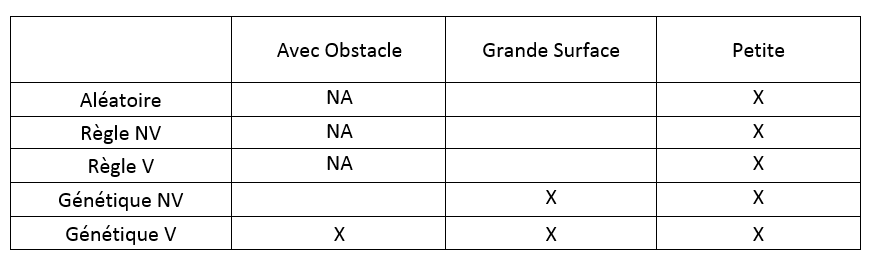
\includegraphics[scale=1]{Consom1}
\end{center}
\begin{center}
	\center
	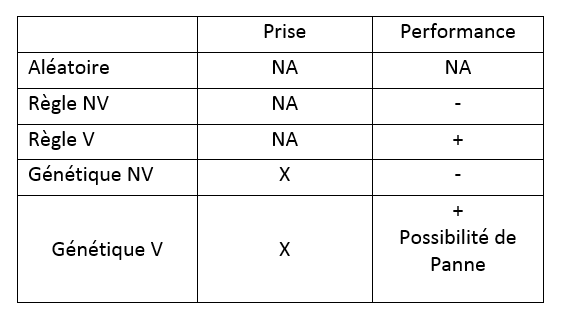
\includegraphics[scale=1]{Consom2}
\end{center}
\begin{center}
	\center
	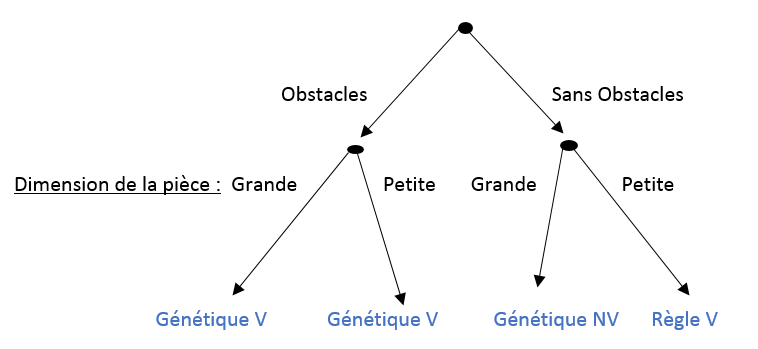
\includegraphics[scale=1]{Consom3}
\end{center}

\section{Intelligence d'un agent artificiel ? }

\section{Conclusion}
\end{document}